\chapter{SPICE Circuit Elements and Device Models}

\label{chap_spicecircuitelementsanddevicemodels_sceadm}

\section{SPICE Suffixes}
\label{subsec_sceadm_suffixes}

These suffixes are used in specifying parameter values for elements.

\begin{tabular}{lll} 
\textit{suffix} & \textit{name} & \textit{magnitude} \\ \hline \\ \vspace{-0.8\parskip}
a & atto- & $10^{-18}$ \\
f & femto- & $10^{-15}$ \\
p & pico- & $10^{-12}$ \\
n & nano- & $10^{-9}$ \\
u & micro- & $10^{-6}$ \\
m & milli- & $10^{-3}$ \\
k & kilo- & $10^{3}$ \\
meg & mega- & $10^{6}$ \\
g & giga- & $10^{9}$ \\
t & tera- & $10^{12}$ \\
\end{tabular}

\clearpage

\section{SPICE Element Identifiers}
\label{subsec_sceadm_elementidentifiers}

The SPICE netlist line for each type of circuit element must start with a specific character.  Here we list the characters all together; examples are presented throughout the rest of this chapter for each element type.

\begin{tabular}{lp{14cm}}
\textit{character} & \textit{element type}\\ \hline \\ \vspace{-0.8\parskip}
\texttt{R} & Resistors (Section \ref{subsec_sceadm_resistors}) \\
\texttt{C} & Capacitors (Section \ref{subsec_sceadm_capacitors}) \\
\texttt{L} & Inductors (Section \ref{subsec_sceadm_inductors}) \\
\texttt{K} & Coupled Inductors (Section \ref{subsec_sceadm_inductors}) \\
\texttt{V} & Independent Voltage Sources (Section \ref{subsec_sceadm_independentsources}) \\
\texttt{I} & Independent Current Sources (Section \ref{subsec_sceadm_independentsources}) \\
\texttt{G} & Voltage-Controlled Current Sources (Section \ref{subsec_sceadm_lineardependentsources}) \\
\texttt{E} & Voltage-Controlled Voltage Sources (Section \ref{subsec_sceadm_lineardependentsources}) \\
\texttt{F} & Current-Controlled Current Sources (Section \ref{subsec_sceadm_lineardependentsources}) \\
\texttt{H} & Current-Controlled Voltage Sources (Section \ref{subsec_sceadm_lineardependentsources}) \\ 
\texttt{B} & Nonlinear Dependent (Behavioral) Sources (Section \ref{subsec_sceadm_behavioralsources}) \\
\texttt{D} & Diodes (Section \ref{subsec_sceadm_diodes}) \\
\texttt{Q} & BJTs (Section \ref{subsec_sceadm_bjts}) \\
\texttt{M} & MOSFETs (Section \ref{subsec_sceadm_mosfets}) \\
\texttt{Z} & MESFETs (Section \ref{subsec_sceadm_otheractiveelements}) \\
\texttt{J} & JFETs (Section \ref{subsec_sceadm_otheractiveelements}) \\
\texttt{S, W} & Switches (Section \ref{subsec_sceadm_switches}) \\
\texttt{T} & Transmission Lines (Section \ref{subsec_sceadm_transmissionlines}) \\

\end{tabular}

\section{Passive Elements}
\label{sec_sceadm_passiveelements}

\subsection{Resistors}
\label{subsec_sceadm_resistors}

\textbf{\textit{Syntax:}}

\spicesyntax{\begin{tabular}{ll}
RXX & [N+] [N-] [VAL] [INLINE PARAMS]
\end{tabular}
}

\begin{longtable}{l l}
\textit{parameter} & \textit{description} \\ \hline \\ \vspace{-0.8\parskip}
\texttt{[N+]} & Positive node/net \\
\texttt{[N-]} & Negative node/net \\
\texttt{[VAL]} & Resistance \\
\texttt{[INLINE PARAMS]} & \begin{tabular}{lp{5.5cm}p{5cm}}Inline parameters \\ 
																					{\small m : Current multiplication factor} \\ 
																					{\small ac : AC value} \\
																					{\small scale : Current scale factor} \\
																					{\small temp :  Temperature} \\
																					{\small dtemp : Temperature difference with ambient} \\
																					{\small tc1 : Linear temperature coefficient} \\
																					{\small tc1 : Quadratic temperature coefficient} \\
																					{\small noisy : Noise on/off}\end{tabular} 
\end{longtable}

\textbf{\textit{Schematics Editor Library:}}

Analog

\textbf{\textit{Schematics Editor Symbol:}}

\begin{figure}[htb]
  \begin{center}
    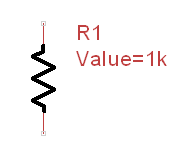
\includegraphics[width=0.15\textwidth]{./pics/SpiceEl/Resistor.png}
  \end{center}
	%\caption{Resistor symbol}
\end{figure}

\textbf{\textit{Schematics Editor Option:}}

"\textsf{Value}" is for assigning an alphanumeric number to \texttt{[VAL]}

\textbf{\textit{Examples:}}

\begin{longtable}{l l}
\textit{statement} & \textit{explanation} \\ \hline \\ \vspace{-0.8\parskip} 
\texttt{r1 1 0 1K} & {\small Insert resistor r1, with resistance 1K$\Omega$, between nets 1 and 0} \\
\texttt{r1 1 0 1K m=2 scale=3} & {\small Insert resistor r1, with resistance 1K$\Omega \times \frac{3}{2}$, between nets 1 and 0}
\end{longtable}

\textbf{\textit{Remarks:}}

"\textsf{Value}" can be set to a model as described next by the alternative syntax. These alternatives can be used by editing the netlist using the netlist editor.
\newline\noindent
{\color{darkgreen}
\textbf{\textit{Alternative Syntax 1:}}

\spicesyntax{\begin{tabular}{ll}
RXX & [N+] [N-] [VAL] [MODEL] [INLINE PARAMS]
\end{tabular}
}

\begin{longtable}{l l}
\textit{parameter} & \textit{description} \\ \hline \\ \vspace{-0.8\parskip}
\texttt{[N+]} & Positive node/net \\
\texttt{[N-]} & Negative node/net \\
\texttt{[VAL]} & Resistance \\
\texttt{[MODEL]} & Resistor model defined by a .model statement \\
\texttt{[INLINE PARAMS]} & \begin{tabular}{lp{5.5cm}p{5cm}}\textit{Inline parameters :} \\ 
																					{\small m : Current multiplication factor} \\ 
																					{\small ac : AC value} \\
																					{\small scale : Current scale factor} \\
																					{\small temp :  Temperature} \\
																					{\small dtemp : Temperature difference with ambient} \\
																					{\small tc1 : Linear temperature coefficient} \\
																					{\small tc2 : Quadratic temperature coefficient} \\
																					{\small noisy : Noise on/off}\end{tabular} 
\end{longtable}

\textbf{\textit{Example:}}

\begin{longtable}{l l}
\textit{statement} & \textit{explanation} \\ \hline \\ %\vspace{-0.1\parskip} 
			\parbox{15em}{\texttt{r1 1 0 1K res tc1=0.01}\\ 
			\texttt{.model res R m=2}}
			& \parbox{25em}{{\small Insert resistor r1, with resistance 1K$\Omega \times \frac{1}{2}$, between\\nets 1 and 0}} 
\end{longtable}

\textbf{\textit{Alternative Syntax 2: Semiconductor resistor}}

\spicesyntax{\begin{tabular}{ll}
RXX & [N+] [N-] [MODEL] [INLINE PARAMS]
\end{tabular}
}

\begin{longtable}{l l}
\textit{parameter} & \textit{description} \\ \hline \\ \vspace{-0.8\parskip}
\texttt{[N+]} & Positive node/net \\
\texttt{[N-]} & Negative node/net \\
\texttt{[MODEL]} & Resistor model defined by a .model statement \\
\texttt{[INLINE PARAMS]} & \begin{tabular}{lp{5.5cm}p{5cm}}\textit{Inline parameters :} \\ 
																					{\small l : Length} \\
																					{\small w : Width} \\
																					{\small m : Current multiplication factor} \\ 
																					{\small ac : AC value} \\
																					{\small scale : Current scale factor} \\
																					{\small temp :  Temperature} \\
																					{\small dtemp : Temperature difference with ambient} \\
																					{\small noisy : Noise on/off}\end{tabular} \\
\texttt{[MODEL PARAMS]} & \begin{tabular}{lp{5.5cm}p{5cm}}\textit{Model parameters :} \\ 
																					{\small tc1 : Linear temperature coefficient} \\
																					{\small tc2 : Quadratic temperature coefficient} \\
																					{\small rsh : Sheet resistance} \\
																					{\small defw : Default width} \\
																					{\small narrow : Width narrowing value} \\
																					{\small short : Length shortening value} \\
																					{\small tnom : Nominal temperature} \\
																					{\small kf : Flicker noise coefficient} \\
																					{\small af : Flicker noise exponent} \\
																					{\small r (res) : Default value} \\
																					\end{tabular}																			
\end{longtable}

\textbf{\textit{Example:}}

\begin{longtable}{l l}
\textit{statement} & \textit{explanation} \\ \hline \\ %\vspace{-0.8\parskip} 
		\parbox{15em}{\texttt{r1 1 0 res l=2u w=1u} \\
			\texttt{.model res R (rsh=10\\+narrow=0.1u short=0.05u)}} 
			& \parbox{25em}{{\small Insert resistor r1, with resistance 10$\times\frac{2u-0.05u}{1u-0.1u}\Omega$,\\between nets 1 and 0}} 
\end{longtable}

\textbf{\textit{Alternative Syntax 3: Behavioral resistor}}

\spicesyntax{\begin{tabular}{ll}
RXX & [N+] [N-] R= { [EXPRESSION] } 
\end{tabular}
}

\begin{longtable}{l l}
\textit{parameter} & \textit{description} \\ \hline \\ \vspace{-0.8\parskip}
\texttt{[N+]} & Positive node/net \\
\texttt{[N-]} & Negative node/net \\
\texttt{[EXPRESSION]} & An equation or expression containing voltages or currents 																	
\end{longtable}

\textbf{\textit{Example:}}

\begin{longtable}{l l}
\textit{statement} & \textit{explanation} \\ \hline \\ %\vspace{-0.8\parskip} 
		\texttt{r1 1 0 r={v(2)*0.1}} 
			& {\small Insert resistor r1, with resistance v(2)$\times$0.1$\Omega$, between nets 1 and 0} 
\end{longtable}
}




\subsection{Capacitors}
\label{subsec_sceadm_capacitors}

\subsection{Inductors}
\label{subsec_sceadm_inductors}

\textit{\textbf{Coupled Inductors}}

\subsection{Behavioral Models}
\label{subsec_sceadm_behavioralmodels}

{\Large etc....}

\section{Sources}
\label{sec_sceadm_sources}

\subsection{Independent Sources}
\label{subsec_sceadm_independentsources}

\subsection{Linear Dependent Sources}
\label{subsec_sceadm_lineardependentsources}

\subsection{Behavioral Sources}
\label{subsec_sceadm_behavioralsources}

\begin{longtable}{c c}

\hline\hline %inserts double horizontal lines
Function Name & Description \\ [0.5ex] % inserts table
%heading
\hline % inserts single horizontal line
abs(x) & Absolute value of x \\ \\ % inserting body of the table

absdelay(x, del), delat(x, del) & \begin{minipage}{20em}
Value of x del amount of independent units before the current value of the independent variable. If the independent variable is less than the delay parameter del zero.
\end{minipage}\\ \\

arcsin(x), asin(x), arccos(x),\\ 
acos(x), arctan(x), atan(x) & \begin{minipage}{20em}
Inverse trigonometric functions. Note these functions give the real part only.
\end{minipage}\\ \\

asinh(x), acosh(x), atanh(x) & \begin{minipage}{20em}
Inverse hyperbolic trigonometric functions. Note these functions give the real part only.
\end{minipage}\\ \\

atan2(y, x) & \begin{minipage}{20em}
Fourth quadrant inverse tangent of y$/$x
\end{minipage}\\ \\

buf(x) & \begin{minipage}{20em}
(x$>$0.5) ? 1.0 : 0.0
\end{minipage}\\ \\

ceil(x) & \begin{minipage}{20em}
Smallest integer that is greater than or equal to x
\end{minipage}\\ \\

dd(x) & \begin{minipage}{20em}
ddt(x) derivative of x against the independent variable
\end{minipage}\\ \\

exp(x) & \begin{minipage}{20em}
e$\rm{^x}$
\end{minipage}\\ \\

floor(x), int(x) & \begin{minipage}{20em}
Largest integer that is less than or equal to x
\end{minipage}\\ \\

hypot(x, y) & \begin{minipage}{20em}
sqrt((x$\rm{^2}$) + (y$\rm{^2}$))
\end{minipage}\\ \\

idt(x[,o[,r]]), sdt(x[,o[r]]) & \begin{minipage}{20em}
Integral of x against the independent variable. 'o' is an optional offset parameter. 'r' is an option reset parameter. If 'r' is true the integral resets to 'o'.
\end{minipage}\\ \\

inv(x) & \begin{minipage}{20em}
(x$>$0.5) ? 0.0 : 1.0
\end{minipage}\\ \\

limit(x, y, z) & \begin{minipage}{20em}
If y $\leq$ x then x, If x $<$ y $<$ z then y, if x $<$ y and z $\leq$ y then z.  
\end{minipage}\\ \\

ln(x), log(x) & \begin{minipage}{20em}
Natural log of x
\end{minipage}\\ \\

log10(x) & \begin{minipage}{20em}
Log base ten of x
\end{minipage}\\ \\

max(x, y) & \begin{minipage}{20em}
x $>$ y ? x : y
\end{minipage}\\ \\

min(x, y) & \begin{minipage}{20em}
x $<$ y ? x : y
\end{minipage}\\ \\

pow(x, y) & \begin{minipage}{20em}
x raised to the power of y (pow from C runtime library)
\end{minipage}\\ \\

pwr(x, y) & \begin{minipage}{20em}
pow(fabs(x),y), note that this function gives only the real part of the answer
\end{minipage}\\ \\

pwrs(x, y) & \begin{minipage}{20em}
sgn(x)$\cdot$abs(x)$\rm{^y}$
\end{minipage}\\ \\

pwl(x, $\rm{x_1,y_1, x_2,y_2}$...) & \begin{minipage}{20em}
Piecewise linear function where the answer value y, is interpolated base on the pair of points between which x falls.
\end{minipage}\\ \\

rand(x), random(x) & \begin{minipage}{20em}
Randomly generated real number y such that \\0 $<$ y $<$ 1 depending on the integer value of x
\end{minipage}\\ \\

round(x) & \begin{minipage}{20em}
Round to nearest integer, x.5 rounds up.
\end{minipage}\\ \\

sgn(x) & \begin{minipage}{20em}
1.0 for x $>$ 0, 0.0 for x equal to 0, -1.0 for x $<$ 0 
\end{minipage}\\ \\

sin(x), cos(x), tan(x) & \begin{minipage}{20em}
Trigonometric functions
\end{minipage}\\ \\

sinh(x), cos(x), tanh(x) & \begin{minipage}{20em}
Hyperbolic trigonometric functions
\end{minipage}\\ \\

sqrt(x) & \begin{minipage}{20em}
y=$\sqrt{\rm{x}}$, note that this function gives only the real part of the answer
\end{minipage}\\ \\

%table(x, x1,y1, x2,y2, ... ) & \begin{minipage}{20em}
%Piecewise linear function where the answer value y, is interpolated base on the pair of points between which x falls.
%\end{minipage}\\ \\

ternary\_fcn(x, y, z), if(x, y, z) & \begin{minipage}{20em}
x ? y : z
\end{minipage}\\ \\

u(x) & \begin{minipage}{20em}
Unit step, x $>$ 0 ? 1 : 0
\end{minipage}\\ \\

unif(nom, rvar) & \begin{minipage}{20em}
Nominal value plus relative variation (to nominal) uniformly distributed between $\pm$rvar
\end{minipage}\\ \\

uramp(x) & \begin{minipage}{20em}
x $>$ 0 ? x : 0
\end{minipage}\\ \\

white(x) & \begin{minipage}{20em}
Randomly generated number y such that -0.5 $<$ y $<$ 0.5
\end{minipage}\\ \\[1ex] % [1ex] adds vertical space
\hline %inserts single line

\caption{Behavioral source functions}
\label {tab:paramfuncs}
\end{longtable}

\section{Active Elements}
\label{sec_sceadm_activeelements}

\subsection{Diodes}
\label{subsec_sceadm_diodes}

\subsection{BJTs}
\label{subsec_sceadm_bjts}

\subsection{MOSFETs}
\label{subsec_sceadm_mosfets}

\subsection{Other Active Elements}
\label{subsec_sceadm_otheractiveelements}

\textbf{\textit{JFETs}}


\textbf{\textit{MESFETs}}



\section{Other Elements}
\label{sec_sceadm_otherelements}

\subsection{Switches}
\label{subsec_sceadm_switches}

\subsection{Transmission Lines}
\label{subsec_sceadm_transmissionlines}

\section{Built-in Subcircuits and Behavioral Elements in CoolSPICE}
\label{sec_sceadm_builtinsubcircuits}

\subsection{Probes}
\label{subsec_sceadm_probes}

Probes, which are found in the \textsf{Analog} library of CoolSPICE, are described in detail in Section \ref{subsec_satco_savestatement}, which is about their associated \texttt{.save} statement.  

\subsection{The \texttt{.include} Statement}
\label{sec_sceadm_includestatement}

\subsection{The \texttt{.subckt} Statement and Subcircuit Definition}
\label{sec_sceadm_subcktstatement}

